%% NOTES TO SELVES
%% ---------------
%% - This is the first paper that discusses how to be systematic about coordinate freedom in ML.
%% - HOGG: Carry the example of FINANCE through everything here, just to make sure we have non-physics examples everywhere. It has both coordinate and units considerations.
%% - BEFORE ARXIV ADD ACKNOWLEDGEMENT INCLUDING BEN BLUM SMITH
%% - decide if we should keep the glosary; HOGG is currently a NO

\documentclass{article}
\usepackage{microtype}
\usepackage{graphicx}
% \usepackage{booktabs} % for professional tables

% hyperref makes hyperlinks in the resulting PDF.
% If your build breaks (sometimes temporarily if a hyperlink spans a page)
% please comment out the following usepackage line and replace
% \usepackage{icml2023} with \usepackage[nohyperref]{icml2023} above.
\usepackage{hyperref}

% Attempt to make hyperref and algorithmic work together better:
\newcommand{\theHalgorithm}{\arabic{algorithm}}

% Use the following line for the initial blind version submitted for review:
\usepackage{icml2023}

% If accepted, instead use the following line for the camera-ready submission:
% \usepackage[accepted]{icml2023}

% For theorems and such
\usepackage{amsmath}
\usepackage{amssymb}
\usepackage{mathtools}
\usepackage{amsthm}

% if you use cleveref..
% \usepackage[capitalize,noabbrev]{cleveref}

%%%%%%%%%%%%%%%%%%%%%%%%%%%%%%%%
% THEOREMS
%%%%%%%%%%%%%%%%%%%%%%%%%%%%%%%%
\theoremstyle{plain}
\newtheorem{theorem}{Theorem}[section]
\newtheorem{proposition}[theorem]{Proposition}
\newtheorem{lemma}[theorem]{Lemma}
\newtheorem{corollary}[theorem]{Corollary}
\theoremstyle{definition}
\newtheorem{definition}[theorem]{Definition}
\newtheorem{assumption}[theorem]{Assumption}
\theoremstyle{remark}
\newtheorem{remark}[theorem]{Remark}

% Todonotes is useful during development; simply uncomment the next line
%    and comment out the line below the next line to turn off comments
%\usepackage[disable,textsize=tiny]{todonotes}
\usepackage[textsize=tiny]{todonotes}

% add our our own custom macros
\usepackage{amsmath}
\usepackage{amssymb}
\usepackage{tikz-cd}
\tikzcdset{every label/.append style = {font = \normalsize}}
\newcommand{\documentname}{\textsl{Article}}
\newcommand{\sectionname}{Section}
\newcommand{\secref}[1]{\sectionname~\ref{#1}}
\newcommand{\bernhard}[1]{~B: \textcolor{red}{\textbf{#1}}}
\newcommand{\inv}{^{-1}}
\newcommand{\T}{^\top}
\newcommand{\R}{{\mathbb R}}
\newcommand{\surf}{{\mathrm{s}}}
\newcommand{\unit}[1]{\mathrm{#1}}
\newcommand{\kg}{\unit{kg}}
\newcommand{\m}{\unit{m}}
\newcommand{\s}{\unit{s}}

% The \icmltitle you define below is probably too long as a header.
% Therefore, a short form for the running title is supplied here:
\icmltitlerunning{~ \hfill Passive symmetries make every machine-learning problem equivariant \hfill \thepage}
\frenchspacing\sloppy\sloppypar\raggedbottom
\begin{document}

\twocolumn[
\icmltitle{Passive symmetries make every machine learning problem equivariant}

\icmlsetsymbol{equal}{*}

\begin{icmlauthorlist}
\icmlauthor{Firstname1 Lastname1}{equal,yyy}
\icmlauthor{Firstname2 Lastname2}{equal,yyy,comp}
\icmlauthor{Firstname3 Lastname3}{comp}
\icmlauthor{Firstname4 Lastname4}{sch}
\icmlauthor{Firstname5 Lastname5}{yyy}
\icmlauthor{Firstname6 Lastname6}{sch,yyy,comp}
\icmlauthor{Firstname7 Lastname7}{comp}
%\icmlauthor{}{sch}
\icmlauthor{Firstname8 Lastname8}{sch}
\icmlauthor{Firstname8 Lastname8}{yyy,comp}
%\icmlauthor{}{sch}
%\icmlauthor{}{sch}
\end{icmlauthorlist}

\icmlaffiliation{yyy}{Department of XXX, University of YYY, Location, Country}
\icmlaffiliation{comp}{Company Name, Location, Country}
\icmlaffiliation{sch}{School of ZZZ, Institute of WWW, Location, Country}

\icmlcorrespondingauthor{Firstname1 Lastname1}{first1.last1@xxx.edu}
\icmlcorrespondingauthor{Firstname2 Lastname2}{first2.last2@www.uk}

% You may provide any keywords that you
% find helpful for describing your paper; these are used to populate
% the "keywords" metadata in the PDF but will not be shown in the document
\icmlkeywords{Machine Learning, ICML}

\vskip 0.3in
]

% this must go after the closing bracket ] following \twocolumn[ ...

% This command actually creates the footnote in the first column
% listing the affiliations and the copyright notice.
% The command takes one argument, which is text to display at the start of the footnote.
% The \icmlEqualContribution command is standard text for equal contribution.
% Remove it (just {}) if you do not need this facility.

%\printAffiliationsAndNotice{}  % leave blank if no need to mention equal contribution
\printAffiliationsAndNotice{\icmlEqualContribution} % otherwise use the standard text.

\begin{abstract}
This purely conceptual paper extends the applicability of group-equivariant methods in machine learning to almost all of machine-learning.
Any representation of data involves arbitrary investigator choices.
Because those choices are external to the data-generating process, each choice leads to an exact symmetry, corresponding to the group of transformations that takes one possible representation to another.
These are the \emph{passive symmetries}; they include coordinate freedom, gauge symmetry, and units covariance, all of which have led to important results in physics.
The passive symmetries strongly constrain mechanistic or causal models, and appear in essentially all data-analysis tasks.
\bernhard{Too much detail for the abstract: The permutation equivariance enforced by graph neural network architectures is an example of a passive symmetry.}
Our goal is to understand how passive symmetries might be used to improve machine learning methods.
We develop conditions under which implementing exact passive symmetries will help (or not help) a learning problem, and we provide examples.
We argue that they are generally helpful, and can be implemented as group equivariances, except when there are relevant hidden constants that are not included among the features in the learning problem. 
Even when there are hidden constants, in some cases they can be learned.
We draw a connection between this point and causal inference.
We argue that 
the implementation of passive symmetries is most valuable when the goal of the learning problem is to generalize out of sample, but they will help in many circumstances.\bernhard{I feel this could be condensed by a third at least, shall I have a go?}
\end{abstract}

\section{Introduction}\label{sec:intro}

Many important ideas in machine learning have come from---or been inspired by---mathematical physics.
These include the kernel trick \cite{CouHil53,SchSmo02} and the use of statistical mechanics techniques to solve probabilistic problems (CITE).
Here we suggest another connection between physics and machine learning, which relates to representation and group theory:
When features and labels (or physics objects) are represented in a mathematical form that involves investigator choices, the machine-learning method (or physical law) must be written in a form that is exactly equivariant to changes in those investigator choices.
These ideas appear in the physics literature as early as Einstein (HOGG CITE), and they are stated in the introduction of Weyl's book as a motivation to study the classical groups \cite{weyl}. More recently, \citealt{mcp} explain in the first sentence of {\em Modern Classical Physics}  
\begin{quote}
..., a central theme will be a Geometric Principle: The laws of physics must all
be expressible as geometric (coordinate-independent and reference-frame-independent)
relationships between geometric objects (scalars, vectors, tensors, ...) that represent
physical entities.
\end{quote}
\bernhard{How about formulating this in a theorem environment and calling it the Geometric Principle?}
This principle leads to the important physical symmetries of coordinate freedom, gauge symmetry, and units covariance.
Each of these symmetries has led to extremely important results in physics. Some of these ideas are exploited in machine learning in the geometric deep learning literature CITE. 
We argue---in this purely conceptual contribution---that analogs of these symmetries could have big impacts in machine learning, and enormously increase the scope of group-equivariant methods in machine learning.

In natural science there are two types of symmetries (see, for example, Section 4.1 of \citealt{rovelli2000loop}). 
The first kind is \emph{passive}, arising from the arbitrariness of the mathematical representation described above.
The second is \emph{active}, empirically established by observations and experiments (including the symmetries that imply the fundamental conservation laws, like momentum, energy, and angular momentum).
Both of these types of symmetries can (often) be expressed in terms of group actions and equivariances, but the epistemological content and range of applicability are very different. 

The redundancies in the representations and parameterizations of the world imply a large set of symmetries.
Mathematically, this can be formulated as invariances or equivariances with respect to changes of arbitrary choices.
One example familiar to machine learners is the equivariance of functions on graphs to the relabeling of the graph nodes.
This is an exact, passive symmetry, described by a permutation group \bernhard{maybe more precise: "by the {\em symmetric group}, consisting of all permutations"}:
If the graph nodes are relabeled or reordered, nothing of significance about the graph changes.
Graph neural network architectures (GNNs) build this passive symmetry in by design.
That has been important and useful in machine learning and it is the source of lines of research regarding expressive power of GNNs (SOLE CITE).

One example familiar to physicists is what we call \emph{units covariance}, which is the requirement that any correct description of the world have inputs and outputs with the correct units.
This is a purely passive, exact symmetry---the choice of units is an arbitrary investigator choice---but the symmetry leads to {\em dimensional analysis}, which is a powerful tool for solving physics problems.
We discuss this example in more detail in \secref{sec:units}.

HOGG: Put this into the next paragraph: Related work coming later.

In this primarily conceptual contribution, we elucidate the passive symmetries and argue that they apply to essentially all data analysis problems \bernhard{that ingest data based on physical measurements}.
They have implications for how we structure machine-learning methods.

\paragraph{Our contributions:}
\begin{itemize}
\item
We introduce active and passive symmetries in the context of machine learning. This is an old concept in classical physics but it hasn't been applied to ML much yet.
\item
We give a formal definition of passive symmetries in terms of group actions and explain how passive symmetries are always in play in all data problems.
\item
We demonstrate with toy examples how enforcing passive symmetries can improve regressions. 
\item
We demonstrate that imposing passive symmetries can lead to the discovery of important hidden objects in a data problem.
\item
We draw two connections with causal inference. One is that all causal graphs and mechanistic models are constrained to be consistent with the passive symmetries. The other is that the determination that a data problem has all the inputs necessary to express the symmetry exactly looks like a causal inference.
\item 
We provide guidance on how to structure machine learning models so that they respect the passive symmetries. We call out some current standard practices that prevent models from obeying symmetries. 
% \item
% We provide a glossary that can be used to translate ideas between physics and machine learning. 
\end{itemize}

\section{Passive symmetries}\label{sec:informal}

This contribution is about the passive symmetries, which arise from redundancies or free parameters or investigator choices in the representation of data.
They are to be contrasted with the active symmetries, which arise from observed or empirical invariances of the laws of physics with respect to continuous parameters, like position, velocity, or angle.
Passive symmetries can be established with no need of observations, as they arise solely from the principle that the physical world is independent of the mathematical choices we make to describe it.
The groups involved in coordinate freedom can be large and complicated (for example, the group of reparameterizations).

In contrast to the passive symmetries, the active symmetries of the Universe are the ones that must be established experimentally.
The laws of physics do not seem (at current precision) to depend on position, orientation, or time, which in turn imply conservation of momentum, angular momentum and energy (according to Noether's Theorem; \citealt{noether}).
These results are empirical results.
Unlike the passive symmetries, active symmetries can be falsified by experimental tests.
 
A big part of the literature on equivariant machine learning is implicitly or explicitly looking at what we call \emph{active symmetries}.
This is possibly because in most problems the coordinate system is fixed before the problem is posed, and both training and test data are expressed in those fixed coordinates, the same for every training-set and test-set datum.
If a data set is made with a fixed coordinate system, but still has an observable invariance or equivariance with respect to (say) rotations then that must represent an active symmetry.
However, these cases of exact, active symmetries are rare; they only really appear in natural-science contexts like protein folding or cosmology.
For example, in a protein folding problem, the way the protein folds does not depend on its orientation (therefore it is actively O(3) equivariant).
This result, in detail, relies on the assumption or observation that the local gravitational force (from the Earth) does not affect the folding.
This is approximately true or assumed or experimentally established; it is an active symmetry.
In contrast, the fact that the protein folds in a way that doesn't depend on the coordinate system chosen to describe it is absolutely and always true; it is not experimentally established; it is a passive symmetry.

The relationship between active and passive symmetries is related to the relationship between what are sometimes called active and passive transformations, or \emph{alibi} and \emph{alias} transformations.
An active or alibi transformation is one in which the objects of study are moved (rotated or translated or interchanged).
A passive or alias transformation is one in which the coordinate system in which the objects of study are described is changed (rotated or translated or relabeled).
Mathematically, the two kinds of transformations seem very similar:
For example, how do we know whether we rotated all the vectors in our problem by $30\,\deg$, or else rotated the coordinate system we are using by $-30\,\deg$?
The answer is that if you rotated \emph{absolutely all} the vectors in your problem, including possibly many latent physical vectors, then there would be no mathematical difference.
But in real problems, where some vectors can't be actively rotated (think, for example of the local gravitational-field vector, or the vector pointing towards the Sun), the two kinds of transformations are different in practice.
In the example above, the rotation of the protein is an active or alibi transformation.
The rotation of the coordinate system describing the protein is a passive or alias transformation.

The protein-folding example suggests that it's very hard to implement or enforce a true passive symmetry in a real data-analysis problem.
It requires us to incorporate all relevant contextual information.
How do we know if all relevant features are part of our data set?
We could perform the protein-folding experiment in a closed, isolated environment to make sure no external forces are in play;
this is impossible for many practical applications, and furthermore there could still exist fundamental constants that are not part of our model or knowledge (see \secref{sec:experiments} and \secref{sec:applicability}).
Another approach is to perform the experiment multiple times after actively putting the molecules into different orientations.
If the protein folds differently in every case, we learn that the problem is not symmetric with respect to the 3d coordinates of the molecule, and therefore when a rotation is performed there must be at least one more vector that needs to be rotated as well (for instance, the gravity vector or the eigenvectors of a stress tensor, say).
This identification of all necessary inputs to establish the passive symmetry is similar to the problem of performing interventions to learn the existence of confounding factors in causal inferences.
We will come back to the connections to causality in \secref{sec:causality}.

We argue that machine-learning methods that do not respect passive symmetries are doomed to make important kinds of mistakes.
We say more about this in \secref{sec:dos}

\section{Example: Units covariance}\label{sec:units}

Consider a mass $m$ near the surface of the Earth, in a location where the surface of the Earth can be considered as a horizontal plane, and close enough to the surface such that the gravitational field can be considered to be determined by a constant (not spatially varying) vector with magnitude $g$ and direction downwards.
\textsl{Question~1:}~If this mass $m$ is dropped (released at rest) from a small height $h$ from above the ground, how much time $T$ does it take to fall to the ground?
\textsl{Question~2:}~If this mass $m$ is launched from the surface at a low velocity of magnitude $v$ at an angle $\theta$ to the horizontal, how much horizontal distance $L$ will it fly before it hits the surface again?
Assume that only $m, g, h$ come in to the solution; assume that the height $h$ and the velocity $v$ are both small enough that air resistance, say, can be ignored.
We will return to this seemingly innocuous point below.

The answers to these questions are almost completely determined by dimensional (or units-covariance) arguments.
The mass $m$ has units of $\kg$, the gravitational acceleration magnitude $g$ has units of $\m\,\s^{-2}$, the velocity magnitude $v$ has units of $\m\,\s^{-1}$, the time $T$ has units of $\s$, and the lengths $h$ and $L$ have units of $\m$.
The angle $\theta$ is dimensionless (it can be measured in radians or degrees, say, which can be converted to radians by a dimensionless constant).
The only possible combination of $m, g, h$ that has units of time is $\alpha\,\sqrt{h/g}$, where $\alpha$ is a dimensionless constant, which doesn't depend on any of the inputs.
The only possible combination of $m, g, v, \theta$ that has units of length is $\beta(\theta)\,v^2/g$, where $\beta(\theta)$ is a dimensionless function of only one dimensionless input.
That is, both Questions~1 and 2 can be answered up to a dimensionless constant (or function) without any considerations beyond those of the units of the inputs and outputs, and without any training data.
And both of those answers don't depend in any way on the input mass $m$, which is a fundamental observation \cite{gr}.

This shows that the structure of physical law can sometimes be inferred from units covariance only, which is a purely passive symmetry.
SOLE: Units covariance has been introduced to machine-learning methods in \cite{villar2022dimensionless, 
SOLE-OTHERS}.
As expected, it helps with training, predictive accuracy, and especially out-of-sample generalization.
The out-of-sample generalization arises because the enforcement of the symmetry enforces scaling properties of the learned function.
These, in turn, help make predictions when the inputs at test time are outside the range of the training data.

This passive symmetry---and all passive symmetries---can deliver information pertaining to the (hard problem of) inference of causal structure:
treating $g$ as a constant, we can construct a structural causal model with the following vertices: (a)~an initial value of $v$, (b)~a value of $m$, chosen independently, and (c)~a final value of $L$, affected by a noise term $\theta$.
Time ordering implies that possible causal arrows are from $v, m, \theta$ to $L$.
As argued above, dimensional analysis rules out the arrow $m\to l$, leaving us with the non-trivial result that in the causal graph, only $v,\theta$ cause $L$.
Again, this conclusion can be reached without any training data or interventions.

That said, there is a strong assumption in play, which is that all relevant quantities for predicting $L$ have been specified in the list $m, g, v, \theta$.
Indeed, the dimensional argument relies strongly on this assumption.
For example, if the projectile is large enough or the speed $v$ is high enough, air resistance will come into play, and the size of the object and the density of air will enter, bringing new variables and new combinations of variables that matter to the answer.
This difficulty is related to the problem in causal inference of knowing or specifying all possible confounding variables.
There is a missing-information problem with all of the passive symmetries, as we discuss below.

\section{Formal definition}\label{sec:definitions}

Consider $\mathcal X$ to be the state space of a specific physical system (for instance $x\in \mathcal X$ could be the positions, velocities, masses, spins, and charges of a set of particles at a given time). 
We consider a family of maps $\{\Phi_i: \mathcal X \to \mathcal H_i\}_{i\in \mathcal I}$ where $\{\mathcal H_i$ is a space of observations or encodings (for instance $\Phi_i(x)$ could be the total mechanical energy of the system $x$ measured in Joules, and $\Phi_j(x)$ could be the momentum of the center of mass, etc).
The family of maps $\{\Phi_i\}_{i\in \mathcal I}$ not only describes the possible observables but also a way to express those observables in a specific coordinate system and with specific units. 

We say that two encodings $\Phi_i$ and $\Phi_j$ are compatible if there exists an invertible morphism $\beta_{j}^i:\Phi_i(\mathcal X)\to  \Phi_j(\mathcal X)$ that makes the diagram commute \eqref{eq.diagram}.
\begin{equation}\label{eq.diagram}
\begin{tikzcd}[]
  {\cal X}\arrow[r,"id"] \arrow[d,"\Phi_i",swap] & {\cal X}  \arrow[d,"\Phi_j"]\\
{\mathcal H} \arrow[r,"\beta_{j}^i"]  & {\mathcal H} 
\end{tikzcd}
\end{equation}

{\tiny
TMP from our e-mail discussion:
\begin{equation}\label{eq.diagram-active-passive}
\begin{tikzcd}[]
  {\cal X}\arrow[r,"T"] \arrow[d,"\Phi",swap] & {\cal X}  \arrow[d,"\Phi_T"]\\
{\mathcal H} \arrow[r,"id"] & {\mathcal H} 
\end{tikzcd}
\end{equation}
}


%Namely, the encodings $\Phi_i$ and $\Phi_j$ are compatible (or \emph{equivalent}) if they express the same aspect of the world in possibly different representation. WE SHOULD FURTHER DISCUSS THIS POINT. For instance in under this definition if $\Phi_i(x)$ is the p 

The passive symmetries are the groupoid of invertible morphisms $\beta$ between compatible encodings that make the diagram commute $\mathcal P = \{\beta: \Phi_i(\mathcal X) \to \Phi_j(\mathcal X) \text{ s.t. } \beta\circ \Phi_i = \Phi_j, \, i,j\in \mathcal I \}$, where the groupoid operator is the composition. We note that this is a groupoid and not a group because not every pair of transformations are composable. 

The groupoid $\mathcal P$ consists of all the possible changes of coordinates or automorphisms between encodings or observables.

Critical to the definition is that we establish beforehand the space of possible observables or encodings $\mathcal H$ and the class of invertible morphisms $\beta$ of $\mathcal H$. For instance, $\mathcal H$ can be in the category of smooth manifolds with smooth diffeomorphisms, or in the category of vector spaces with invertible linear transformations.   

For example take $\mathcal X$ to be a space of proteins, the $\Phi_i$  could be the list of positions of each of its atoms in some coordinate system. The passive symmetries include reordering of the atoms or changes the coordinate system by any 1-1 transformation. Note that a priori there are no restrictions on the $\beta$'s but for practical purposes we may restrict $\mathcal H$ to the category of smooth manifolds with the $\beta$'s being diffeomorphisms.  

The active symmetries can be thought as transformations of the world that preserve a relationship between two encodings or observations. Given a compatible family of observations $\{\Phi_i\}_{i\in I}$ as above, we say that a 1-1 map $\alpha:\mathcal X \to \mathcal X$ is an active symmetry (for those observations) if there exists $i,j\in I$ such that $\mathcal H_i = \mathcal H_j$ and the diagram  \eqref{eq.diagram2} commutes. 
\begin{equation}\label{eq.diagram2}
\begin{tikzcd}[]
  {\cal X}\arrow[r,"\alpha"] \arrow[d,"\Phi_i",swap] & {\cal X}  \arrow[d,"\Phi_j"]\\
{\mathcal H} \arrow[r,"id"]  & {\mathcal H} 
\end{tikzcd}
\end{equation}

%If $\Phi_i = \Phi_j$ the active symmetry is an invariance with respect to the group 


SOLE: REWRITE THIS SECTION
When the transformations $\alpha$ and $\beta$ are actions by a certain group, then both active and passive symmetries can be expressed in terms of group equivariances.
They are useful in machine-learning models \cite{cohen2016group, kondor2018convolution, thomas2018tensor, geiger2022e3nn, finzi2020generalizing, finzi2021practical} and have scientific applications \cite{batzner20223, musaelian2022learning, stark2022equibind, yu-physics, wang2022approximately}.
Equivariant machine-learning models can predict the properties and behaviour of physical systems (as argued in \citealt{cheng2019covariance}), with the correct inductive bias, achieving smaller generalization error \cite{bietti2021sample, elesedy2021provably, elesedy2021kernel, mei2021learning} and allowing for out-of-distribution generalization \cite{villar2022dimensionless}. 
Even the non-trivial diffeomorphism symmetries of general relativity have been considered for machine learning \cite{weiler}.

%\bernhard{you have commented out the next two paragraphs in the latex file -- maybe let's discuss?}

Imposing a passive symmetry on the structure of a machine-learning model can permit the discovery of scalings, structures, or missing elements in the physical description of, or predictions about, the problem.
We illustrate these ideas with some toy examples below.
The passive symmetries are seemingly trivial statements about the world, but they lead to strong constraints on the laws of physics, and deliver scaling arguments that solve real problems in physics.
They can constrain machine learning in valuable ways.
\emph{We conjecture that enforcing passive symmetries in machine learning and data-analysis tasks will lead to generalization improvements in a wide range of circumstances.}
In particular, we make this conjecture even for problems in which no (or few) active symmetries are present.
After all, most problems (like reading handwriting or predicting gravitational trajectories near the surface of the Earth) are not equivariant to rotations, reflections, and translations, but they are all, in their data-generating processes, exactly coordinate free.

\section{Experiments and examples}\label{sec:experiments}

\paragraph{Black-body radiation}
An important moment in the history of physics was the discovery by Planck that the electromagnetic radiation intensity $B_\lambda$ (energy per time per area per solid angle per wavelength) of thermal black-body radiation can be described with a simple equation \cite{planck}
\begin{equation}
    B_\lambda(\lambda) = \frac{2\,h\,c^2}{\lambda^5}\,\frac{1}{\exp\frac{h\,c}{\lambda\,k\,T} - 1}~,
\end{equation}
where $h$ is Planck's constant,
$c$ is the speed of light,
$\lambda$ is the wavelength of the electromagnetic radiation,
$k$ is Boltzmann's constant,
and $T$ is the temperature.
In finding this formula, Planck had to posit the existence (and units) of the constant $h=6.6\times 10^{-34}\,\kg\,\m^2\,\s^{-1}$ (Planck's original value was presented in $\mathrm{erg}\,\s$, which are different units but the same dimensions).
Prior to the introduction of $h$, the only dimensionally acceptable expression for the black-body intensity was $B_\lambda(\lambda)=2\,c\,k\,T/\lambda^4$, which is the long-wavelength (infrared) or high-temperature limit.
Planck's discovery solved the ``ultraviolet catastrophe'' of classical physics.
This is the problem that, classically, the black-body spectrum, or any thermal object, ought to contain infinite numbers of excited modes at short wavelengths, or high frequencies, and thus infinite energy density.
Planck's solution seeded the development of quantum mechanics, which governs the behavior of all matter at small scales, and which cuts off the ultraviolet modes through quantization of energy.

Planck's problem can be solved almost directly with the passive symmetry of units covariance.
That is, the exponential cut-off of the intensity appears at a wavelength set by the temperature and a new constant, that must have units of action (or action times $c$, or action divided by $k$, or one of a restricted set of other options).
We have shown (SOLE MAKE APPROPRIATE REFERENCE HERE TO THE EXPERIMENTS SHOWN AND DESCRIBE THEM), with a simple toy training set, that no units-covariant regression for the intensity as a function of $\lambda, T, c, k$ can reproduce accurately the intensity $B_\lambda$, but that when the regression is permitted to introduce a new dimensional constant (but remain units covariant given the new constant), it finds a constant with units (and, less precisely, magnitude) that is consistent with $h$ (or $h$ times a combination of $c$ and $k$).
Again, this shows that the passive symmetry leads to powerful capability.

\begin{figure*}
    \centering
    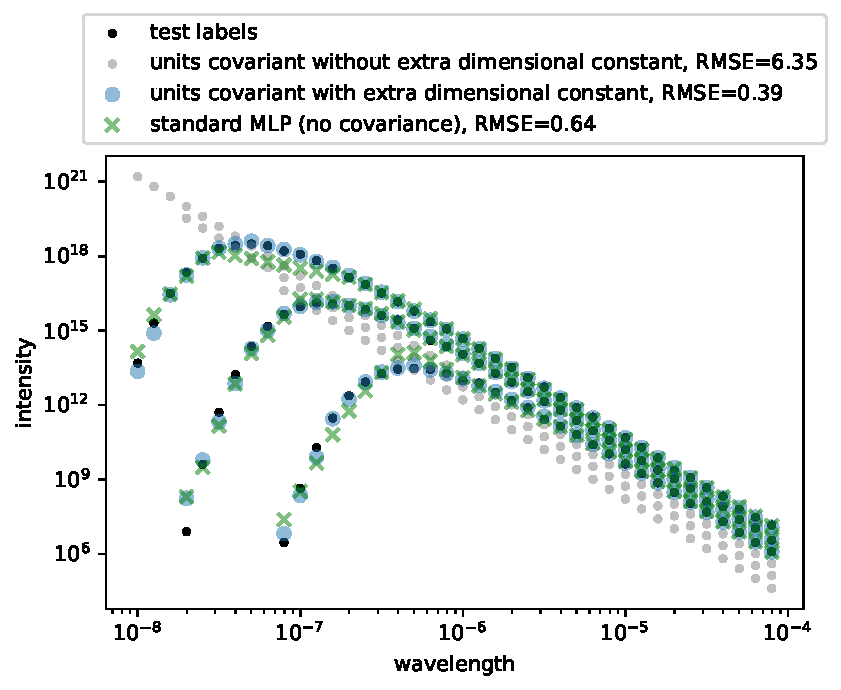
\includegraphics[height=0.3\textwidth]{units}
    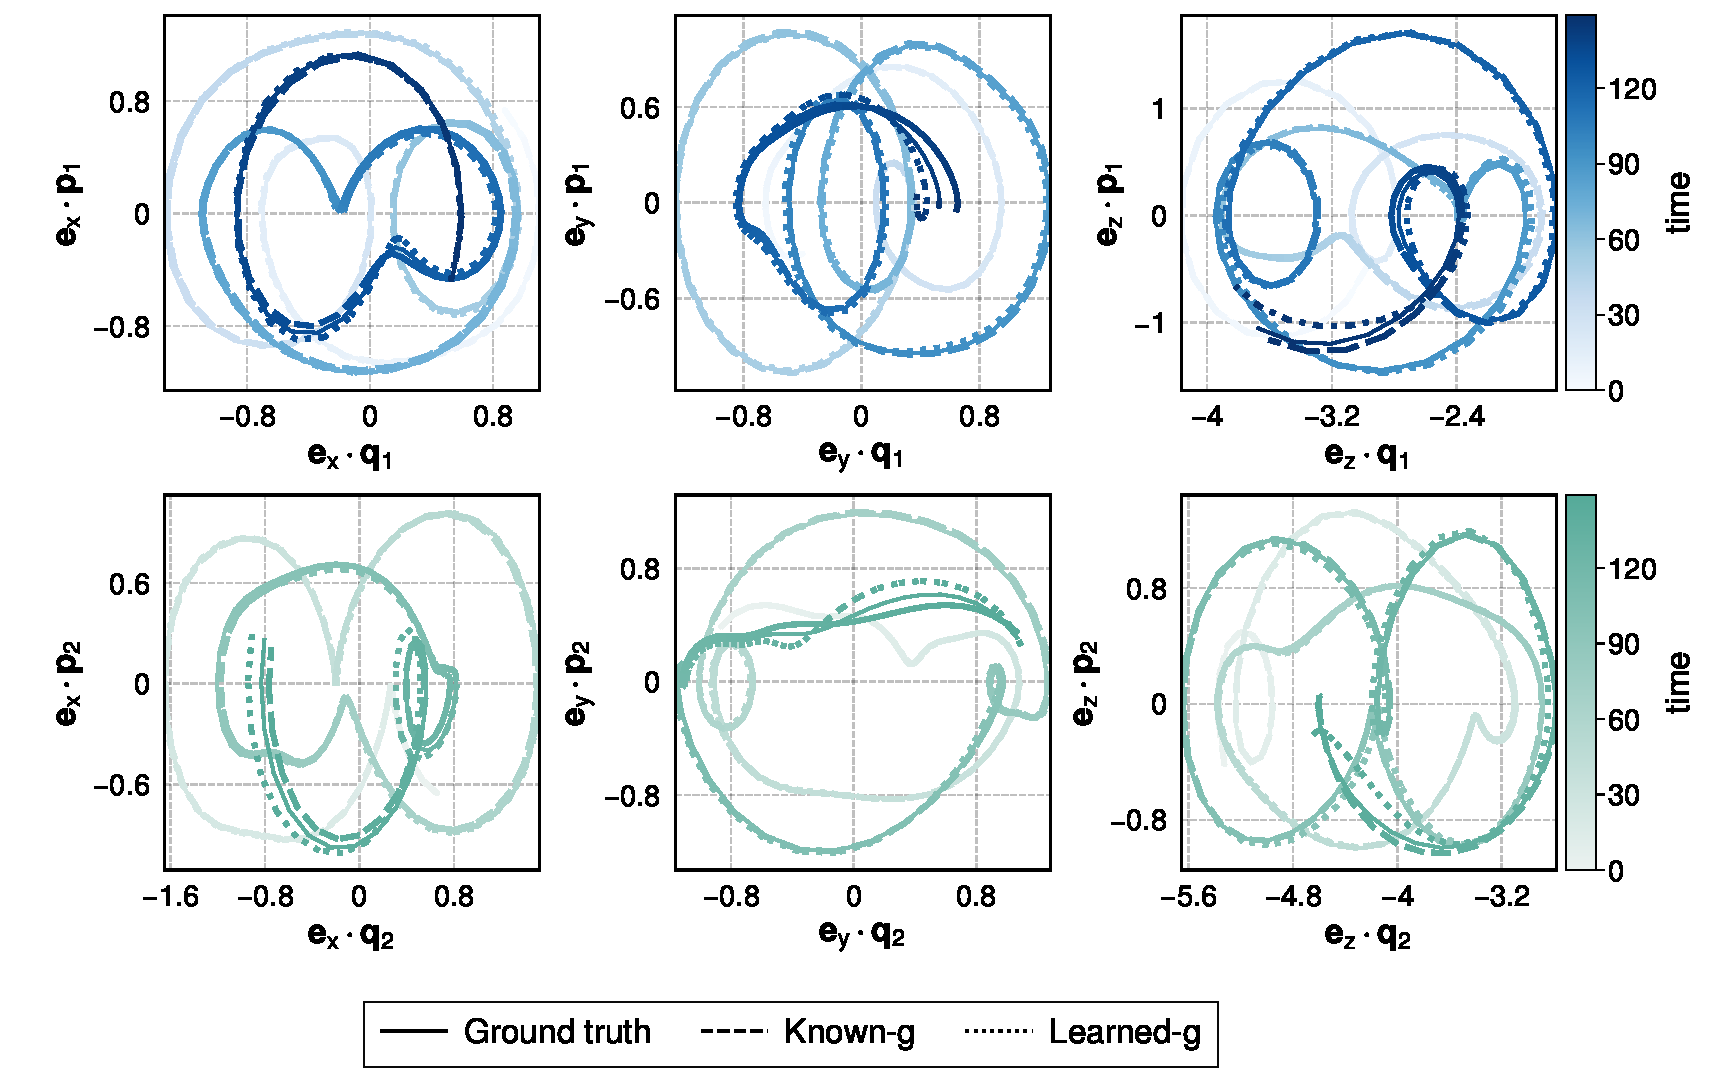
\includegraphics[height=0.3\textwidth]{pendulum}
    
    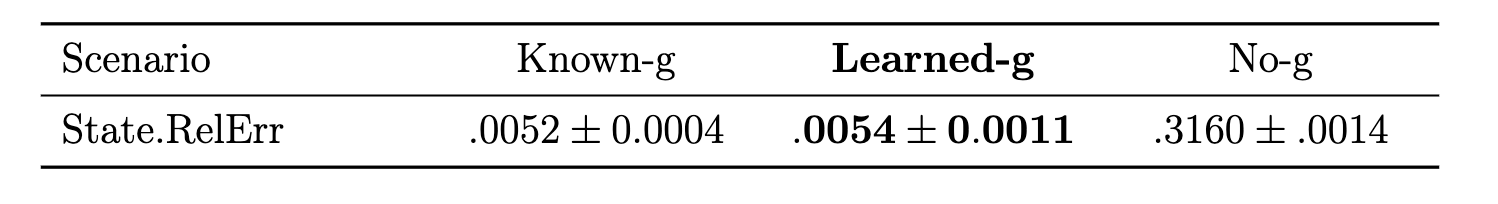
\includegraphics[width=0.5\textwidth]{table}
    \caption{Caption}
    \label{fig:my_label}
\end{figure*}

\paragraph{Springy double pendulum}

The double pendulum connected by springs is a toy example often used in equivariant machine-learning demonstrations \cite{finzi2021practical,yao2021simple}. 
The final conditions (position and velocities of both masses after elapsed time $T$) are related to the initial conditions (position and velocities of the masses at the initial time), and the dynamics is classically chaotic.
The vectors are 3-dimensional, subject to a passive $O(3)$ equivariance, but the problem contains an \emph{active} $O(2)$ equivariance (the dynamics is equivariant with respect to rotations and reflections in the 2-d plane normal to gravity).
The $O(3)$ symmetry is passive, because it is guaranteed by the fact that all vectors must be described in a coordinate system; nothing physical can change as the vectors undergo passive or alias transformations because of coordinate-system changes.
The $O(2)$ symmetry is active, because it is an experimental fact that if the initial conditions are changed by an active or alibi rotation in the plane perpendicular to gravity, the dynamics and final state rotate accordingly.
It was shown in \cite{yao2021simple} that when the problem is treated with a machine-learning method that is restricted to be equivariant to the full passive $O(3)$ symmetry, training and generalization are improved over the case in which the method is restricted only to be equivariant for the smaller active $O(2)$ symmetry.
That is, even though the dynamics of the double pendulum contains an explicit spatial anisotropy, the existence of the passive $O(3)$ symmetry is powerful for model structure and generalization.
Indeed, the passive symmetry is more powerful than the active symmetry.

In that problem, $O(3)$ symmetry was implemented by converting the network inputs (which are scalars and components of vectors) into invariant scalar quantities according to the Einstein summation rules (which explicitly encode $O(3)$ symmetry), building the nonlinear machine-learning model in the space of the invariant scalars, and multiplying back to input vectors to make the output predictions (as per \citealt{villar2021scalars}).
That is, the machine-learning model was restricted to use structures that are invariant to the $O(3)$ group action.
This restriction on model capacity is significant, even though the problem does not have $O(3)$ symmetry in the active sense.
Later, the passive symmetry of units covariance was also applied to this problem, and generalization improved even further \cite{villar2022dimensionless}.

\section{Connections with causality}\label{sec:causality}

BS: Spell out the connection to causality---both the trivial point that causal and mechanisitic relationships are also (obviously) covered by these passive symmetries, and more subtle or interesting things??

BS: The idea of homomorphic structure \eqref{eq.diagram} in the representation space $\cal H$ also applies to causal world models (eg, the brightness changes in the real world may be represented as retinal gain control mechanisms in the nervous system; \citealt{1911.10500}).
 Other instantiations of the commutative diagram \eqref{eq.diagram} include representations that retains the dimensions of system components but drops all numbers, \bernhard{add: representations that drops the dimensions and only retains numeric values,} or the representation that converts systems into physical equations.

\bernhard{New: There is another intriguing connection to causality that we have glossed over above.
We made the assumption that only quantities come into the solution (in our case, $m, g, h$). How would we ascertain such an assumption in practice; e.g., why does temperature not affect the result? In essence, this is not a probabilistic statement, but one about the behavior of a system under experimentation, i.e., intervention. A set of experiments can indicate that a certain outcome (or effect variable) depends on a certain set of input (cause) variables but is independent of certain other potential cause variables. The physical law is thus not inferred from dimensional arguments alone, but from a combination of dimensional and causal arguments.}

\bernhard{This is also related to the issue of transfer: in practice, we may not be able to tell all inputs (and non-inputs) from experimentation. E.g., it is nontrivial to intervene on $g$ (unless we can run an experiment in an elevator, say). However, we may know from having previously solved a related problem that we expect a problem to depend on $g$. This is a form of qualitative transfer which we believe may be relevant in practice.}

\section{Connections to current ML practice}\label{sec:practice}

Most machine learning implementations don't impose exact symmetries, but sometimes they promote approximate invariances or equivariances typically by means of data augmentation (see CITE). In this \documentname we focus on the exact symmetries: Given data spaces $X$ and $Y$ and a group $G$ acting on $X$ and $Y$, equivariant machine learning restricts the hypothesis space to a space of functions $\mathcal F$ satisfying  $f(g\cdot x) = g \cdot f(x)$ for all $f\in \mathcal F$, $g\in G$, $x\in X$. There are two main approaches to perform optimization in the space of equivariant functions:
\begin{itemize}
    \item Explicitly parameterizing the space of equivariant functions via equivariant layers or weight sharing CITE.
    \item Finding a set of invariant features and expressing the invariant/equivariant functions in terms of those features.
\end{itemize}

SOLE: Move text here about prior work, about implementations, about results on 

\section{Dos and Don'ts}\label{sec:dos}

MacKay famously wrote ``Principal Component Analysis is a dimensionally invalid method that gives people a delusion that they are doing something useful with their data. If you change the units that one of the variables is measured in, it will change all the `principal components'\,'' (in a now-deleted comment on an Amazon review \citealt{muldoonmedium}).
This comment is aligned with our mission here, but also slightly wrong: If a rectangular data set contains only data with identical units (that is, all features of all records have the same units), then PCA does excactly the right thing.
That said, if a rectangular data set has features with different units (for example, if every record contains a position, a temperature, a voltage, and a few intensities), then indeed the output of PCA will be extremely sensitive to the units system in which the features are recorded.
If PCA is run on such a data set, the subsequent data model or data manipulations will be, by construction, asymmetric or not consistent with the passive symmetry of units covariance.
The choice to use PCA on such a data set is the choice to be wrong.

Similarly, consider a kernel function that returns elements of a kernel matrix given inputs that are lists of features.
If the kernel function involves, say, the exponential of the sum of squares of the differences of the input features, the output of the kernel function cannot obey the passive symmetry of units covariance.
Quantities with different units cannot be summed, and dimensional (as opposed to dimensionless) quantities cannot be exponentiated.

Learning involves optimization.
Optimization is of a scalar cost function (a number, which is a function of many parameters).
If passive geometric groups are in play, like $O(3)$, the parameters that are explicitly or implicitly components of vectors can only be combined into the scalar objective through the Euclidean norm.
Otherwise the scalar objective isn't scalar in the geometric sense of ``invariant to $O(3)$'', and the optimization won't return a result that is invariant (or equivariant) to $O(3)$.
Similarly, if the components of the vector are normalized differently before they are summed in quadrature, the objective won't be invariant to $O(3)$.
And similarly, if all the different contributions to the objective aren't converted to the same units before being combined into the objective, then the model won't be units covariant.
The common practices of making objectives with functional forms other than Euclidean norm, normalizing features with data ranges, and combining features with different units, all make common machine-learning methods, by construction, inconsistent with the passive symmetries in play.

L1 and L-infinity norms are almost always inconsistent with the passive symmetries.
This is because the sum of absolute values of input components, and the maximum of inputs, are rarely either geometrically, or from a units perspective, covariant.
There is a rare exception if all features have the same units, and none of the features are components of geometric objects.

Transcendental functions like \texttt{exp()} and \texttt{arctanh()} can only be applied to scalars---that is, not components of vectors or tensors but geometric scalars---and only dimensionless scalars.
That means that the nonlinearities in neural networks are predicated on the weights removing the units of the input features, and the linear combinations performing some kind of dot products on the inputs.
That, in turn, means that the internal weights in neural networks implicitly both have geometric properties and units.
They have the geometric properties and units such that the latent variables passed into the nonlinear functions are dimensionless scalars.
There are exceptions:
If the nonlinearity is mathematically homogeneous, as it is for a pure monomial, or for the unmodified RELU function, dimensional scalars (but not vector or tensor components) can be taken as inputs.

\section{Discussion}\label{sec:discussion}

SOLEDAD: MERGE THESE NEXT FEW POINTS INTO DISCUSSION

In order for passive symmetries to be useful one needs to incorporate all relevant constants to the training data. If there exists unknown constants $K$ then the passive symmetry in play is the subgroup that fixes $K$.

Example: the double pendulum is O(3)-equivariant if the gravity vector is part of the training data. If the gravity vector is not part of the training data then the double pendulum is invariant with respect to the subgroup of O(3) that fixes the gravity vector, namely O(2). The space invariant of functions in both cases coincide.

Example: if the model is missing dimensional constants then 

   Changing the coordinate system allows you to conjecture the existence of hidden constants and maybe to find them. 
   
   The formulation of the symmetry poses the existence of the hidden constant. This can be posed as a completeness argument. Including the constant allows for formulating the system with the full symmetry.
   Identifiability issues may arise when more constants are present.
   
   We shouldn't get into the area of learning the problem. 

HOGG: MAKE SURE WE DISCUSS THE places where this most helps us! We claim in the abstract.


DISCUSSION
In this conceptual \documentname,
we argued that passive symmetries are in play in essentially all machine-learning or data-analysis tasks.
They are exact, and true by definition, since they emerge from the redundancies or freedom in coordinate systems, units, or data representation.
Enforcement of these symmetries should improve enormously the generalization capabilities of machine-learning methods.
We demonstrated this with a few toy examples.

In practice, implementation of the passive symmetries in a machine-learning problem might be very difficult.
One reason is that the symmetries are only exact when all relevant problem parameters (including often fundamental, unvaried constants) are known and included in the learning problem.
These pieces of essential contextual information can be hard to find or learn; in our toy examples they include the Planck constant (for the blackbody-radiation problem) and the gravitational acceleration vector (for the double-pendulum example).
Another reason is that some kinds of symmetries are hard to enforce.
For example, complete coordinate diffeomorphisms and problem reparameterizations involve enormous groups which are hard to implement in a realistic machine-learning method.
That said, many groups have been implemented usefully, including translations, rotations, permutations, and changes of units. HOGG / SOLE CITES HERE.

% - SOLE: DO WE NEED TO MENTION AND CITE Equivariant Representation learning (https://arxiv.org/abs/2012.02771)? Here or somewhere above in Related Work?

In addition to the exact (and true by definition) passive symmetries, and the observed active symmetries, there are other kinds of approximate or weakly broken symmetries we might call \emph{observer symmetries}.
These arise from the point that the content of a data record (an image, say) is independent of the minor choices made by the observer in taking that data record (shooting the image, say).
The details of the six-axis location and orientation of the camera, and of the exposure time and focues, can be changed without changing the semantic or label content of the image.
These symmetries are approximate, because of course these changes don't lead to invertible changes to the recorded data; there is no group or groupoid in the space of the data.
However, the success of convolutional structure in image models might have to do with the importance of these observer symmetries.
There is much more to do in this space.

{\raggedright
\bibliography{example_paper}
\bibliographystyle{icml2023}
}

\newpage\appendix\onecolumn
\section{Glossary}
\paragraph{symmetry}
Given a mathematical object $X$ of any sort, (like a manifold, metric space, equation, etc), any mapping of the object onto itself that preserves the corresponding structure is a \emph{symmetry}.

\paragraph{representation}
There are two meanings of the word \emph{representation}. One is the approximate way we describe a system (or all the objects in a system) either in a mathematical model or on a computer.
The other is the \emph{representation of a group} $G$: a homomorphism $\rho: G\to \text{GL}(V)$ where $V$ is a vector space and $\text{GL}(V)$ denotes the space of invertible linear transformations from $V$ to itself.

\paragraph{equivariance}
Let $G$ be a group that acts on vector spaces $X$ and $Y$ as $\rho_X$ and $\rho_Y$ respectively. We say that a function $f:X\to Y$ is \emph{equivariant} if for any group element $g\in G$ and any possible input $x$, the function obeys $f( \rho_X(g) x) = \rho_Y(g)\cdot f(x)$.
The actions of $G$ in $X$ and $Y$ induce an action on the space of maps from $X$ to $Y$. If $f\in \text{Maps(X,Y)}$ then $g\cdot f = \rho_Y(g)\circ f \circ \rho_X(g)^{-1}$.
The equivariant maps are the fixed points of this action.
Equivariances define symmetries in the space of maps. 

\paragraph{invariance}
An equivariance in which the action in the output space is trivial is called an \emph{invariance}.

\paragraph{coordinate freedom}
When physical quantities are measured, or represented in a computer, they must be expressed in some coordinate system.
The redundancy of this representation---the fact that the investigator had many choices for the coordinate system---leads to a symmetry, which is known as \emph{coordinate freedom}:
If the inputs to a physics problem are moved to a different coordinate system (because of a change in the origin or orientation), the outputs of the problem must be correspondingly moved.

\paragraph{covariance}
When a physical law is written in a way that is consistent with the geometric principle, then the law is sometimes said to be \emph{covariant}.

\paragraph{general covariance}
The covariance of relevance in general relativity \cite{einstein} is known as \emph{general covariance}.
Because general relativity is a metric theory in $3+1$ spacetime dimensions with invariance with respect to arbitrary diffeomorphisms, this is a very strong symmetry.
General covariance is sometimes called ``coordinate freedom'', but it is a special case thereof.

\paragraph{conservation law}
We say that a quantity obeys a \emph{conservation law} if changes in that quantity (with time) inside some closed volume can are quantitatively explained by fluxes of that quantity through the surface of that volume.
\emph{Active} (not passive) symmetries lead to conservation laws in dynamical systems \cite{noether}.

\paragraph{units}
All physical quantities are measured with a system of what we call \emph{units}.
A quantity can be transformed from one unit system to another by multiplication with a dimensionless number.
Almost all quantities---including almost all scalars, vectors, and tensors---have units.

\paragraph{units covariance}
The left-hand side and the right-hand side of any equation must have the same units.
This symmetry is called (by us) \emph{units covariance} (contra \cite{villar2022dimensionless}).

\paragraph{gauge freedom}
Some physical quantities in field theories (for example the vector potential in electromagnetism) have additional degrees of freedom that go beyond the choice of coordinate system and units.
These freedoms lead to additional passive symmetries that are known as \emph{gauge freedom}.

\section{HOGG'S HOMEWORK}

HOGG: MOVE THIS TO SECTION 2
{\em Imagine that we want to write a function with inputs that are objects or physical quantities in some representation and an output that is another object or physical quantity in that representation.
We want this function to respect or enforce or exactly obey all passive symmetries that arise from redundancies in representation.
This requirement can be translated into a kind of \emph{equivariance}:
If the representation of the inputs is changed, the representation of the output should change correspondingly.
When the redundancies in representation are expressed by a group action, this equivariance is a group equivariance.

In some ways, the simplest passive symmetry to enforce is that with respect to rotations and reflections of the coordinate system.
This symmetry is an $O(d)$ equivariance, where $O(d)$ is the orthogonal group in the spatial dimension $d$ (often $d=3$).
These symmetries are enforced when all functions are written in accord with the \emph{geometric principle} \cite{mcp}:
This principle states that physical law must be written in terms of vectors, tensors, and coordinate-invariant scalars, and that these objects can only be combined in certain very specific ways.
There are rules for combining scalars, vectors, and tensors into new scalars, vectors, and tensors (sometimes Einstein summation notation, \citealt{einstein}; and sometimes Ricci calculus \citealt{ricci}); they were introduced for making functions equivariant to coordinate diffeomorphisms on curved manifolds.
In summation notation, objects are written in index notation (a scalar has no indices, a vector has one index, and a $k$-tensor has $k$ indices).
Products of objects can have indices summed in pairs (and only pairs), and sums can only be performed among objects with the same number of unsummed indices.
(In the Ricci calculus, there are also considerations of raised and lowered indices, or covariant and contravariant vectors; these considerations are important when the spatial or spatiotemporal metric is non-trivial.)
When the inputs to a function are scalars, vectors, and tensors, and the function conforms to these rules, the function will produce a geometric output (a scalar, vector, or tensor, depending on the number of unsummed indices), and the function will be precisely equivariant to rotations and reflections of the coordinate system.

One consequence of the summation notation is that nonlinear (say) vector functions can always be written as nonlinear functions of (only) scalars and scalar products, times the original input vectors.
See also \cite{villar2021scalars}.
In general, if the equivariance in question is from a group or symmetry with known or easily implemented invariants, then the families of equivariant functions can usually be constructed from the invariants \cite{blum2022equivariant}.
In the case of the $O(d)$ group, scalars (and the scalar products made from vectors and tensors) are the invariants.

Another straightforward implementation is in the area of units covariance:
The objects that are invariant with respect to changes in the units system are the dimensionless quantities.
And indeed, units-covariant functions can be written in terms of nonlinear functions of dimensionless quantities multiplied by dimensional combinations of function inputs that have the same dimensions as the function output \cite{villar2022dimensionless}.

There are many other passive symmetries, including translation and boost, Lorentz, coordinate diffeomorphisms, reparameterizations (including canonical transformations), and gauge.
Some of these are easy to implement and some are difficult.
In general, we recommend looking for invariants of the group action (or invariants of the redundancy) and capitalizing on those invariants.
But there are also implementations that make use of irreducible representations in group theory \cite{fuchs2020se, thomas2018tensor, geiger2022e3nn}.
Not all passive symmetries have practical implementations available at present.

In this \documentname{} we argue that invariances and equivariances are always a desirable property in data-driven models for physics (including machine learning and other forms of regressions).
If the target of a regression is invariant or equivariant, then performing the regression and projecting its outcome onto the space of invariant/equivariant functions results on better generalization (smaller error, smaller sample complexity).
Generalization improvements have been explicitly quantified under different sets of assumptions \cite{bietti2021sample, elesedy2021provably, mei2021learning, elesedy2021kernel}. }


\end{document}


